% The entire content of this work (including the source code
% for TeX files and the generated PDF documents) by 
% Hongxiang Chen (nicknamed we.taper, or just Taper) is
% licensed under a 
% Creative Commons Attribution-NonCommercial-ShareAlike 4.0 
% International License (Link to the complete license text:
% http://creativecommons.org/licenses/by-nc-sa/4.0/).
\documentclass{article}

% My own physics package
% The following line load the package xparse with additional option to
% prevent the annoying warnings, which are caused by the package
% "physics" loaded in package "physicist-taper".
\usepackage[log-declarations=false]{xparse}
\usepackage{physicist-taper}
\makenomenclature % For an index of symbols.

\title{Notes of Group Theory and Physics}
\date{\today}
\author{Taper}


\begin{document}


\maketitle
\abstract{
    Notes of Group Theory and Physics written by Sternberg \cite{Sternberg1994}.
}
\tableofcontents

\section{Basic definitions and examples (Ch 1)}
\label{sec:Basic-def-examples}

    \subsection{The Classification of the finite subgroups of
    \texorpdfstring{$\mathrm{SO}(3)$}{} (1.8)}
    \label{sec:Classif-subg-SO3}

    Previous section established one important formula for this section. Suppose a
    group $G$ acts on a set $M$. Define the \nomen{fix point set}
    $\operatorname{FP}(a)$ of an element $a\in G$ as the set of all $m\in M$ such
    that $am=m$, i.e. left invariant under $a$. Denote \nomen{$G_m$} for $m\in M$ as the
    isotropy subgroup of $m$. Then we have
    \begin{equation}
        \sum_{a\neq e} \#\operatorname{FP}(a) =
        \sum_{\text{orbits}}\frac{\#G}{\#G_m}(\#G_m-1)
        \label{eq:fp-orbit-formula}
    \end{equation}
    The proof is on section 1.7 of \cite{Sternberg1994}.

    This section classifies all possible finite subgroups of $\mathrm{SO}(3)$. The
    classification of finite subgroups of $\mathrm{O}(3)$ is on the next section.
    We basically study the action of $G=\mathrm{SO}(3)$ on $M=S^2$, the unit sphere.
    The first interesting discovery is
    \begin{thm}[(Euler)]
        When the dimension $n$ is odd, any $a\in \mathrm{SO}(n)$ leaves at least one
        non-zero vector invariant, i.e. any $a\in \mathrm{SO}(n)$, $\Ker(a-I)\neq
        \emptyset$, or there is always a $\vb{v}\neq 0$, such that $a\vb{v}=\vb{v}$.
    \end{thm}
    This implies that any rotation in odd dimensional space is a rotation about some
    fixed axis (since $a\vb{v}=\vb{v}$ implies
    $(a\vb{p})\vdot\vb{v}=(a\vb{v})\vdot(a\vb{p})=\vb{v}\vdot\vb{p}=0$).

    Then the book analyses the formula counting fix point sets and
    orbits~\ref{eq:fp-orbit-formula}. Use new symbols for three numbers:
    \begin{table}[H]
        \centering
        \label{tab:three-symbols-for-3-numbers}
        \begin{tabular}{c l}
            $n$ & $=$ $\# G$ \\
            $r$ & $=$ $\text{number of orbits of $G$}$ \\
            $n_i$ & $=$ $\# G_m \text{, where $m\in i$th orbit.}$
        \end{tabular}
    \end{table}

    Then we have
    \begin{equation}
        2-\frac{2}{n} = r-\sum_{1}^{r} \frac{1}{n_i}
    \end{equation}

    This equation can be simplified by considering the practical numerical values of
    $n$, $r$ and $n_i$, with $n_i \leq n$. By eliminating case by case, he finally arrived
    at five sets of possible values:
    \begin{table}[H]
    \centering
    \label{tab:Finite-rot-g}
    \caption{Finite rotation groups}
    \begin{tabular}{l l l l l l}
        \hline
        $r$ & $(n_1,n_2,n_3)$ & $\# G$ & Schoenflies & Hermann-Mauguin & Note
        \\
        \hline
        \hline
        2 & (n,n,0) & n & $C_n$ & $n$ & Cyclic group \\
        3 & $(2,2,k), k\geq 2$ & $2k$ & $D_k$ & $222$ for $D_2$, $k2$ otherwise & Dihedral group \\
        3 & $(2,3,3)$ & 12  & $T$  & 23& of regular tetrahedron \\
        3 & $(2,3,4)$ & 24 & $O$ & 432 & of regular octahedron \\
        3 & $(2,3,5)$ & 60 & $I$ & not mentioned & of icosahedron, of
        Fullerene\footnotemark\\
        \hline
    \end{tabular}
    \end{table}
    \footnotetext{See section 1.10 about Fullerene and icosahedron for details.}
    For details about derivation please visit pp. 28 to 31 of \cite{Sternberg1994}.
    But we need to exclude some subgroups from the list of crystallographic groups.
    The result is that, on the first row, $n$ is restricted to be $1,2,3,4$ and $6$;
    on the second row, $k$ is restricted to be $2,3,4$ and $6$. And $I$ is excluded
    from the list of crystallographic groups. 

    The reason is the common one on Solid States classes about possible space-filling
    polygons (see pp.31 of \cite{Sternberg1994}). Also, a good proof about possible
    rotation angles in three-dimension for a lattice is provided on pp.31 to 32 of
    \cite{Sternberg1994}. The key is that the rotation matrix could be
    made of integers, and hence its characteristic (trace) should be an integer.

    Next the author mentioned the \nomen{atomic hypothesis}, an interesting
    historical account of our view on crystals. The essence is that because only
    above mentioned angles occurred in rotational symmetries of crystals, we can
    presume that a crystal is not a continuum, but is "built up from discrete
    subunits in a regular repetitive pattern" (pp.32).

    He also mentions the \nomen{law of rational indices} which found a basis for
    modern way of labeling different faces of a lattice (the $(100)$ side, etc.).
    But this law is too long to be typed here.

    In sum, we have only following finite subgroups of $\mathrm{SO}(3)$ that is
    interested for crystals:

    $$ C_1, C_2, C_3, C_4, C_6, D_2, D_3, D_4, D_6, T, O $$

    \subsection{Classification of finite subgroups of
    \texorpdfstring{$\mathrm{O}(3)$}{}}
    \label{sec:Classif-subg-O3}
    
    This section based on the work of previous
    section~\ref{sec:Classif-subg-SO3}. To use the result of those groups of
    matrices with $\det=1$ in that section, the author first discuss the
    example of $T_d$ and $O$.

    $T_d$ is the group of all symmetries(including those that does not preserve
    the chirality, i.e. with $\det=-1$) of tetrahedron. As abstract groups,
    $T_d$ and $O$ are all isomorphic to $S_4$, the symmetric group of order $4$.
    Note that in the context of crystal symmetry, the isomorphic class of group is
    not enough to characterize a behavior. For example, the $C_2$
    containing $\pi$ rotation is not the same as $\{e,i\}$ where $i$ is
    the inversion, but they are isomorphic.\footnote{Perhaps representation
    classes of groups is more precise in describing the behavior.} The link
    between $T_d$ and $O$ can be seen from the following:

    \begin{myquote} \enquote{
    we can consider our tetrahedron as situated inside a cube, with its vertices
    at the diagonally opposite vertices of each face of the cube. For a given
    cube there are two such tetrahedra, as shown in Fig. 1.13
    (Figure~\ref{fig:fig1.13} here).
    One tetrahedron is carried into the other by the inversion, $-I$.
    } \end{myquote}
    \begin{figure}[H]
        \centering
        \includegraphics[width=0.6\linewidth]{pics/{fig1.13}.png}
        \caption{Fig 1.13 in \cite{Sternberg1994}, with modification}
        \label{fig:fig1.13}
    \end{figure}

    Written mathematically, we have
    \begin{equation}
        T_d = S_4 = T\cup T'
    \end{equation}
    where $T$ is mentioned in Table~\ref{tab:Finite-rot-g}. And $T'$ contains
    those matrices with $\det=-1$.
    \begin{equation}
        T_d \overset{\phi}{\cong} O
    \end{equation}
    where $\phi$ is defined as
    \begin{align*}
        A \to A\quad &\text{for }A\in T \\
        B \to -B\quad &\text{for }B\in T'
    \end{align*}

    In general case, for a finite subgroup $G$ of $\mathrm{O}(3)$, we have the
    following. Let $G_+$ denote the subgroup of $G$ with positive determinant.
    Let $G_-$ denote the set of elements of $G$ with negative determinant. We
    have two cases.

    Case 1, $-I\in G_-$, then $G_-=(-I)G_+$, and the structure is simple.

    Case 2, $-I\notin G_-$. Then the author defines $G^\vee:=G_+\cup (-I)G_-$,
    and shows that 
    \begin{align}
        G^\vee &= G_+ \cup aG_+ \\
        G_- &= (-I)aG_+
    \end{align}
    where $a$ is some matrix in $G^\vee\setminus G_+$.

    Then,
    \begin{myquote} \enquote{
    From the $11$ rotation groups listed at the end of the preceding section, we
    obtain $11$ non-rotation groups by including $-I$. In addition, we must check for
    the normat subgroups of index two in each rotation group in order to
    construct non-rotation groups which do not include $-I$.
    } \end{myquote}

    The rest of this section carries out this analysis, culminating in the
    table~ 4 on pp. 40 of \cite{Sternberg1994}. I reproduce the table with some
    addition in the Table~\ref{tab:point-g-32}.

    \begin{table}[H]
        \centering
        \caption{The $32$ point groups}
        \label{tab:point-g-32}
        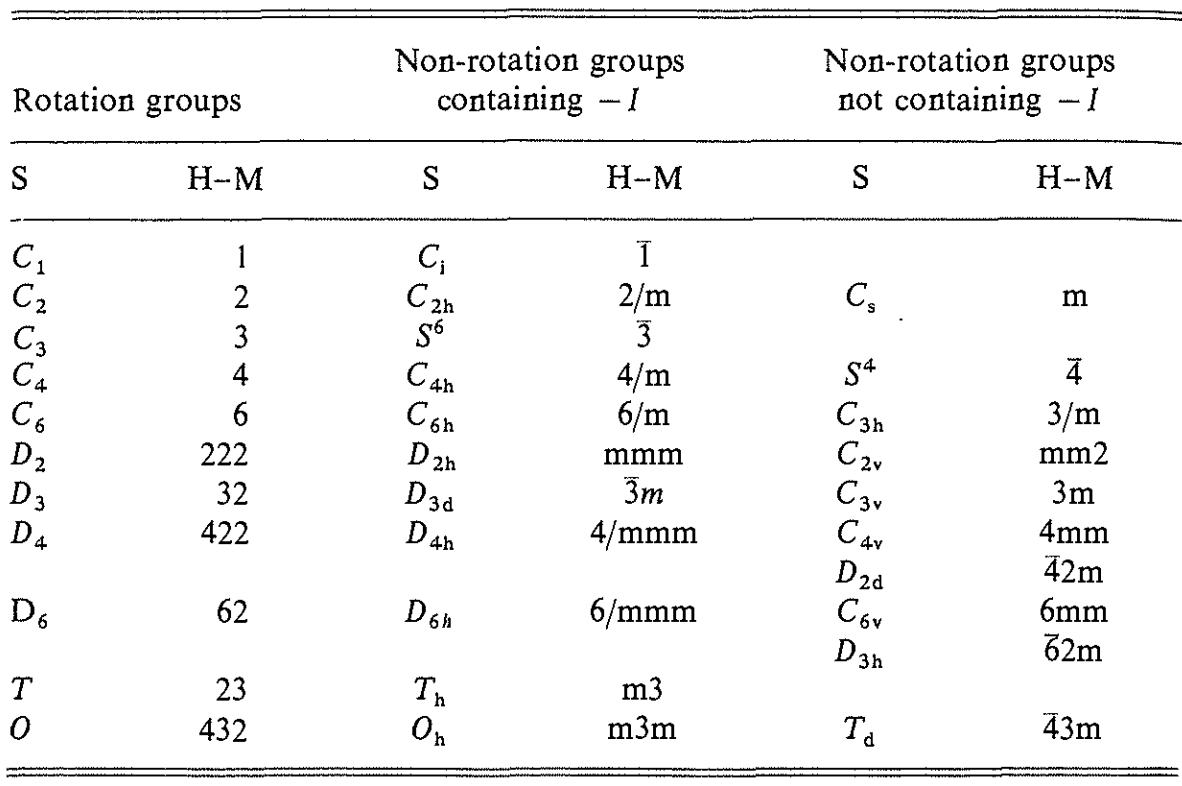
\includegraphics[width=1\linewidth]{pics/table4-32-point-group.png}
    \end{table}

    The detailed derivation could be found on pp.35 to 39 of
    \cite{Sternberg1994}. Note that $S^6\neq S_6$, and $S^4\neq S_4$. Here is
    some explanations for subscripts: 
    \begin{table}[H]
    \centering
    \begin{tabular}{c l}
        $h$: & there is a horizontal reflection plane. \\
        $v$: & there is a vertical reflection plane. \\
        $d$: & there is diagonal vertical planes. \\
        $m$: & there is a vertical mirror plane (in H-M notation). \\
        $/m$: & there is a horizontal mirror plane (in H-M notation).
    \end{tabular}
    \end{table}
    
    Note also that the online engine WolframAlpha is a very good source for
    details about certain groups. For example, this
    \href{http://m.wolframalpha.com/input/?i=crystallographic+point+group+C4h}{link}
    is a good description of group $S^4$ (thouhg it is denoted $S_4$ on the
    webpage). Searching "crystallographic point group C4h" will get one a good
    \href{http://m.wolframalpha.com/input/?i=crystallographic+point+group+C4h}{description}
    of $C_{4h}$. One can also found the book reference from that page by
    clicking the "Source information" link.

    Then the author goes on to mention some historical methods in "determination
    of the actual symmetry groups of a given substance", "available to 19th
    century crystallographers". One method is "to attack the crystal with an
    acid, and to study the etch figures induced on the faces".  Another is to
    study the "piezoelectricity", or to test the "rotatory optical activity".

    He also gives a helpful graphical display of $32$ point groups in Fig 1.19
    on \cite{Sternberg1994}(from pp.42 to 44), which is too long to be included
    here.
\bibliography{cite}
\bibliographystyle{alpha}

\printnomenclature
\section{License}
The entire content of this work (including the source code
for TeX files and the generated PDF documents) by 
Hongxiang Chen (nicknamed we.taper, or just Taper) is
licensed under a 
\href{http://creativecommons.org/licenses/by-nc-sa/4.0/}{Creative 
Commons Attribution-NonCommercial-ShareAlike 4.0 International 
License}. Permissions beyond the scope of this 
license may be available at \url{mailto:we.taper[at]gmail[dot]com}.
\end{document}
